\documentclass{beamer}

\usepackage{helvet}
\usepackage{hyperref, graphicx}
\usepackage{amsthm, amsfonts}
\usepackage{etoolbox}

\usetheme[progressbar=frametitle, numbering=none]{metropolis}
\usecolortheme[snowy]{owl}
\setbeamertemplate{navigation symbols}{}
\AtBeginSection[ ]
{
\begin{frame}{Outline}
    \tableofcontents[currentsection]
\end{frame}
}

% Default fixed font does not support bold face
\DeclareFixedFont{\ttb}{T1}{txtt}{bx}{n}{11} % for bold
\DeclareFixedFont{\ttm}{T1}{txtt}{m}{n}{12}  % for normal - use in headings

% Custom colors
\usepackage{color}
\definecolor{TUGray}{RGB}{101,101,137}
\definecolor{TUBlack}{RGB}{30,0,0}
\definecolor{mygreen}{RGB}{45,111,63}
\definecolor{keywords}{RGB}{205,114,0}
\definecolor{comments}{RGB}{181,51,139}
\definecolor{strings}{RGB}{58,144,81}
\definecolor{numeric}{RGB}{66,110,176}
\definecolor{linos}{rgb}{0.4,0.4,0.4}
\definecolor{links}{rgb}{0,0.4,0.75}

\definecolor{bggray}{RGB}{232, 233, 235}

\setbeamercolor{alerted text}{fg=mygreen}
\setbeamercolor{normal text}{fg=TUBlack}\usebeamercolor*{normal text}

\setbeamercolor{codecol}{fg=TUGray!25!black,bg=bggray}

\hypersetup{colorlinks, linkcolor=links, urlcolor=links}

\usepackage[T1]{fontenc}
\usepackage{fontspec}
\usepackage[sfdefault,scaled=.85]{FiraSans}
\usepackage{newtxsf}

\usepackage{listings}

\newtoggle{InString}{}% Keep track of if we are within a string
\togglefalse{InString}% Assume not initally in string

\newcommand\digitstyle{\color{numeric}}
\makeatletter
\newcommand{\ProcessDigit}[1]
{%
  \ifnum\lst@mode=\lst@Pmode\relax%
   {\digitstyle #1}%
  \else
    #1%
  \fi
}
\makeatother

\lstset{literate=%
    {0}{{{\ProcessDigit{0}}}}1
    {1}{{{\ProcessDigit{1}}}}1
    {2}{{{\ProcessDigit{2}}}}1
    {3}{{{\ProcessDigit{3}}}}1
    {4}{{{\ProcessDigit{4}}}}1
    {5}{{{\ProcessDigit{5}}}}1
    {6}{{{\ProcessDigit{6}}}}1
    {7}{{{\ProcessDigit{7}}}}1
    {8}{{{\ProcessDigit{8}}}}1
    {9}{{{\ProcessDigit{9}}}}1
	{<=}{{\(\leq\)}}1
	{>=}{{\(\geq\)}}1,
	% morestring=[b]",
    % morestring=[b]',
    % morecomment=[l]//,
}

% Python style for highlighting
\newcommand\pythonstyle{\lstset{
language=Python,
basicstyle=\ttfamily\tiny,
numbers=left,
numberstyle=\tiny\color{linos},
morekeywords={self},              % Add keywords here
keywordstyle=\tiny\color{keywords},
commentstyle=\it\tiny\color{comments},    % Custom highlighting style
stringstyle=\tiny\color{strings},
xleftmargin=18pt,
xrightmargin=4pt,
aboveskip=0pt,
belowskip=0pt,
escapeinside={(*@}{@*)},
frame=l,                         % Any extra options here
showstringspaces=false,
keepspaces=true
}}

% Python environment 
\lstnewenvironment{python}[1][]
{
	\pythonstyle
	\lstset{
	#1
	}
}
{}

% wrap the Python environment
\newenvironment{codeblock}
    {\hfill\begin{beamerboxesrounded}[lower=codecol, width=0.8\textwidth]
    \medskip

    }
    { 
    \end{beamerboxesrounded}\hfill
    }

\theoremstyle{example}
\newtheorem{question}{Question}

\newcommand{\ct}[1]{\lstinline[language=Python]!#1!}
\newcommand{\ttt}[1]{{\small\texttt{#1}}}
\newcommand{\lsitem}[2]{\ttt{{#1}[}\ct{#2}\ttt{]}}

\author{Prof.\ Chris Cornwell}
\date{August, 2025}
\title{Day 1 Stuff \\ {\small First lecture - MATH 371}}
\institute{Towson University, Dept.\ of Mathematics}

\begin{document}

\begin{frame}
\titlepage
\end{frame}

%%%%
\begin{frame}
\frametitle{About me}
\begin{itemize}
    \item \textit{Prefer to be called:} Chris or Dr.~Cornwell
    \item \textit{Preferred pronouns:} He/him/his
    \item \textit{Email:} \ttt{ccornwell@towson.edu}
    \item \textit{Office:} YR 227
    \item \textit{Likes:} Enthusiastic about math; like traveling, hiking, soccer, and gaming.
\end{itemize}

\vspace*{24pt}
\pause
If I don't respond quickly to an email or message, it does not mean that I am declining to answer. During the week, I make an effort to return messages within 24 hours. 
\end{frame}

%%%%
\begin{frame}
\frametitle{Office hours}

Please visit office hours. I am happy to discuss questions you have and class topics.

\vspace*{12pt}
\textbf{Regular office hours:} Tuesday 9:00 {--} 10:00 am, Wednesday 1:00 {--} 2:30 pm. Otherwise, please email to make an appointment at another time.

\vfill
\end{frame}

\section{Course structure}

%%%%
\begin{frame}
\frametitle{What is this course about?}
Topics:

\begin{itemize}
	\item[] Fundamentals of machine learning.
    \item[] Basics of Python, implementing machine learning (on data) in Python.
\end{itemize}

\pause
More specifically, we will cover:
\begin{itemize}
    \item A working knowledge of Python.
	\item Foundational \emph{regression} and \emph{classification} machine learning models, including SVM's.
    \pause
	\item Training and testing models.
    \pause
    \item Feature selection.
    \item Some learning theory, avoiding overfitting, and model evaluation.
    \pause
    \item Potentially (time permitting): Tree-based methods or clustering.
\end{itemize}

\end{frame}

%%%%
\begin{frame}
\frametitle{Assignments and Grades}
    \begin{itemize}
        \item Classwork: short, group work ($\sim$ 30 minutes in class). Grading not detailed; more about completion and effort.
        \pause
        \item Homework: $\sim$ 2-3 of these per month. Spend time on these, have discussions about them with each other, with me. Often involve some coding, some mathematical work. 
        \pause
        \item Two midterm exams.
        \item A final project.

        \vfill
        \pause
        \item Grades: 10\% classwork, 30\% homework, 30\% two midterms \mbox{(\textit{15\% each}),} and 30\% final.
    \end{itemize}
    
\end{frame}

%%%%
\begin{frame}
\frametitle{In class}
Some of class will be lecture and we will often have time for group work and coding.
\vspace*{12pt}
%\pause
\begin{itemize}
    \pause
    \item Bring a laptop to class if able; the classroom also has computers available.
    \item I will be available to give direction with group assignments and assigned notebooks.
    \pause
    \item \textit{Occasionally, instead of group work questions we may have questions (given as a poll to class), followed by group discussions.}
\end{itemize}
\end{frame}

%%%%
\begin{frame}
\frametitle{Exams and Project}
\textbf{Exams:} The course has two midterm exams, which will be written by hand. Exam questions will be related to what has been emphasized in class and has been asked on assignments. \newline 
\pause
As an exam date nears, we will discuss what to expect on the exam. 

\vspace*{12pt}
\pause
\textbf{Project:} Students will work on a final project that puts ideas that we discuss this semester into practice. Will work with data provided by Dr.~Joel Moore (Professor of Geosciences) on and related to some chemical properties of water in regional reservoirs. 

\vspace*{12pt}
\pause
\begin{itemize}
    \item Midterm 1: planned for Thursday, October 2.
    \item Midterm 2: planned for Thursday, November 13.
    \item Final projects due: Tuesday, Dec 9.
\end{itemize}
\end{frame}

\section{Course resources}

%%%%
\begin{frame}
\frametitle{Course on Github}
Many class resources will be on the Github repository \href{https://github.com/cornwell/math371-F25}{here}. 

\onslide<2->{
I will place links on Blackboard to some of the folders at that site, including class slides, Jupyter notebooks, and data sets. Check back, they will be updated regularly.
}

\centering
\onslide<1->{
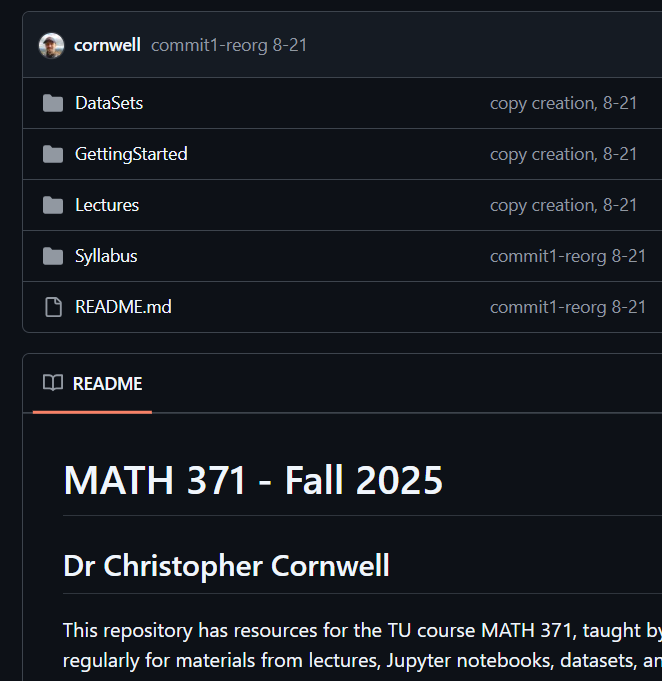
\includegraphics[height=0.65\textheight]{math371-github.png}
}
\end{frame}


%%%%
\begin{frame}
\frametitle{Course on Blackboard}
Screenshot of the course on Blackboard below. Homework will be linked to there, but also available on the class Github repo.

\onslide<2->{Some HW questions require written responses, I will collect in class on the due date.\footnote{My preferred set up. If instead you want everything in one file, please discuss with me.} For HW requiring coding, a Jupyter notebook file, attached in an email to me.
}

\centering
\onslide<1->{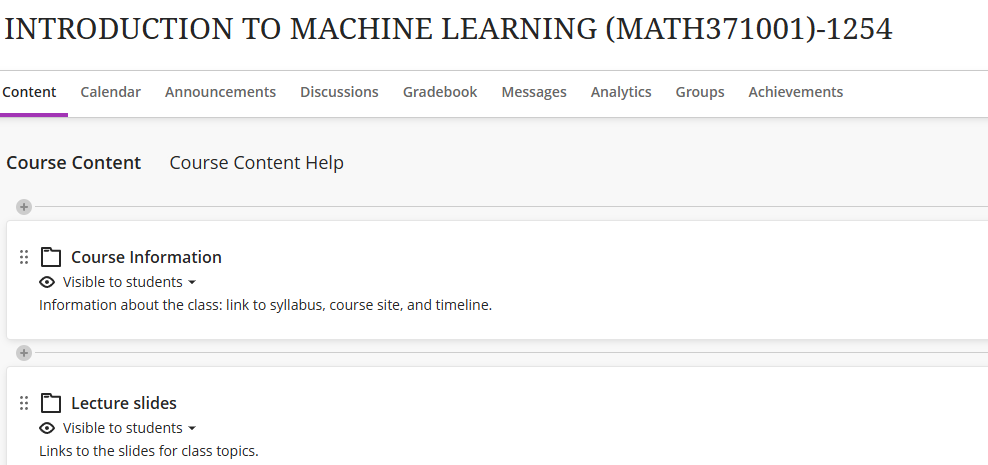
\includegraphics[width=0.8\textwidth]{math371-blackboard.png}
}    
\end{frame}

%%%%
\begin{frame}
\frametitle{Textbook}
I've found a textbook!
\begin{itemize}
    \item \textit{Machine Learning Refined: Foundations, Algorithms, and Applications}, by Watt, Borhani, and Katsaggelos. ({\color{comments}Download from Blackboard})
\end{itemize} 

\pause
Some supplemental textbooks: 

\begin{itemize}
    \item \textit{An Introduction to Statistical Learning: With Applications in Python}, by James, Witten, Hastie, Tibshirani, and Taylor. (\href{https://www.statlearning.com/}{Link})
    \item \textit{Understanding Machine Learning} by Shalev-Shwartz and Ben-David.
    \item \textit{Mathematics for Machine Learning}, by Deisenroth, Faisal, and Ong. (\href{https://github.com/mml-book/mml-book.github.io/blob/master/book/mml-book.pdf}{Link})
%    \item \textit{Deep Learning Book (Part I)}, by Goodfellow, Bengio, and Courville. (\href{https://www.deeplearningbook.org/}{Link})
\end{itemize}

\pause
May provide and assign a few reading excerpts from supplemental texts. Also, will use notes from lectures by Andrew Ng (\href{https://hai.stanford.edu/people/andrew-ng}{website}) and, potentially, Elizabeth Munch (\href{https://elizabethmunch.com}{website}). 
\end{frame}

%%%%
%\begin{frame}
%\frametitle{Discord channel}
%
%When you want
%\vspace*{12pt}
%
%\end{frame}
{\setbeamercolor{palette primary}{fg=mygreen, bg=bggray}
\begin{frame}[standout]
    Questions?
\end{frame}
}

\end{document}